\documentclass[11pt,fleqn]{article} 
\usepackage[margin=1in, head=0.8in]{geometry} 
\usepackage{amsmath,amssymb,latexsym,graphics,fancybox,fancyhdr,graphicx}
\usepackage{fancyhdr} 
\usepackage{palatino, url, multicol}
\usepackage{graphicx} 
\usepackage[all]{xy}
\usepackage{polynom} 
\usepackage{pdfsync}
\usepackage{framed}
\usepackage{pgf,tikz}
\usepackage{enumerate}
\usepackage{amsmath,amssymb,latexsym,graphics,fancybox,fancyhdr,graphicx}
\usetikzlibrary{arrows}
\newcommand{\blankbox}[2]{\fbox{\rule{#1}{0in}\rule{0in}{#2}}}
%		Problem and Part
\newcounter{problemnumber}
\newcounter{partnumber}
\newcommand{\Problem}{\stepcounter{problemnumber}\setcounter{partnumber}{0}
       \item[\fbox{\parbox{.18in}{\hfil\theproblemnumber\hfil}}]}
\newcommand{\Part}{\stepcounter{partnumber}\item[(\alph{partnumber})]}
\newcommand{\Points}[1]{(#1 points) \quad}
\usepackage[margin=1in]{geometry}

\begin{document}
\newcommand{\blank}[1]{\rule{#1}{0.75pt}}
\renewcommand{\d}{\displaystyle}
\vspace*{-0.25in}
\lhead{\sc MAKE UP}
\chead{\Large \sc Math 252X Final Exam} 
\rhead{\sc Fall 2025}
\cfoot{}

%
\small

\thispagestyle{fancy}

\begin{tabular}{l@{\hspace{.2in}}l}
Your Name & \\
\blankbox{2.9in}{.45in} & \\[.1in]
%Student ID \# \\
%\blankbox{.25in}{.25in}%
%\blankbox{.25in}{.25in}%
%\blankbox{.25in}{.25in}%
%\blankbox{.25in}{.25in}%
%\blankbox{.25in}{.25in}%
%\blankbox{.25in}{.25in}%
%\blankbox{.25in}{.25in}
&
\end{tabular}

%\begin{tabular}{l@{\hspace{.2in}}l}
%Start Time & End Time\\
%\blankbox{2.9in}{.45in} & \blankbox{2.9in}{.45in} \\[.1in]
%%Student ID \# \\
%%\blankbox{.25in}{.25in}%
%%\blankbox{.25in}{.25in}%
%%\blankbox{.25in}{.25in}%
%%\blankbox{.25in}{.25in}%
%%\blankbox{.25in}{.25in}%
%%\blankbox{.25in}{.25in}%
%%\blankbox{.25in}{.25in}
%&
%\end{tabular}



{
\renewcommand{\baselinestretch}{1.8}
\setlength{\tabcolsep}{.2in}
\small
\begin{center}
\begin{tabular}{|c|c|c|}
\hline
Page&Total Points&\parbox{.8in}{\hfil Score\hfil}\\
\hline
1&16&\\
\hline
2&12&\\
\hline
3&6&\\
\hline
4&6&\\
\hline
5&4&\\
\hline
6& 10&\\
\hline
7 & 10 & \\
\hline
8 & 8 & \\
\hline
9 & 8 & \\
\hline
10 & 10 & \\
\hline
11 & 10 & \\
\hline
\hline
Total&100&\\
\hline
\end{tabular}

\end{center}
}

\begin{itemize}

\item You will have 2 hours to complete the test.

\item You may bring in 1 page of notes. 
\item No calculators, cell phones, or computers allowed. 
%\item
%You are not allowed to share notes or calculators.
%\item Label any diagrams so as to indicate axes labels and scale.
%\item
%In order to receive full credit, you must {\bf show your work.}  
%Please write out your
%computations on the exam paper.
%\item When a problem asks you to \textbf{set up only} you do NOT need
%  to simplify the integrand (the expression inside the integral sign)
%  at all. 
%\item When determining convergence or divergence of a series, state
%  the test that is being applied. Common abbreviations are
%  acceptable. 
%\textbf{PLACE A BOX AROUND \fbox{YOUR FINAL ANSWER} to each question} where appropriate.

\end{itemize}




 

\newpage
\vspace*{-0.4in}


\begin{enumerate} 
\item (16 points) Evaluate the following integrals. 

\begin{enumerate}
\item $\d \int \sin^3 ( 2 x ) \cos^2 (2 x ) dx$
\vfill

\item $\d \int \frac{x-8}{(2x-1)(x-3)} dx$
\vfill
\newpage
\item $\d \int \arctan \left( \frac{x}{2} \right) dx$ 
\vfill

\item $\d \int \frac{x^2}{(4 - x^2)^{1/2}} dx$
\vfill
\end{enumerate}
\newpage

\item (12 points) Let $R$ be the region bounded by the graph of $f(x) = 1 +
  \sqrt{x}$, $g(x) = e^{-3x}$ and the vertical line $x = 1$, whose
  graphs are given below.  \\
  
  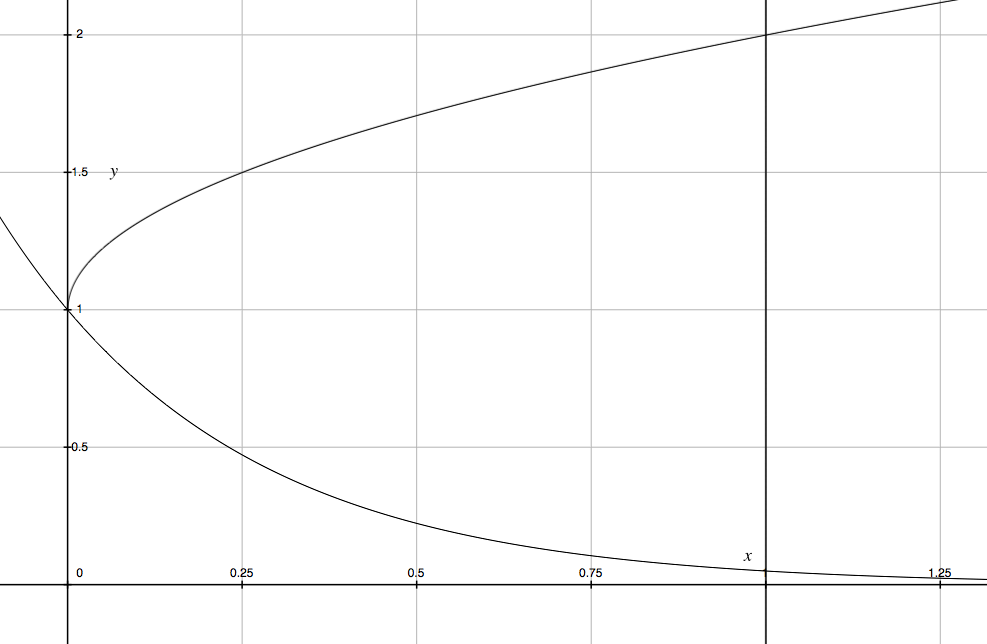
\includegraphics[width=3.5in]{graphs}


  \begin{enumerate}
  \item Set up, but do not solve, an integral that gives the area of
    $R$. 

\vfill

  \item Set up, but do not solve, an integral that finds the volume of
    the solid when $R$ is rotated about the $x$-axis. 
\vfill
  \item Set up, but do not solve, an integral that finds the volume of
    the solid when $R$ is rotated about the $y$-axis. 
\vfill
 \end{enumerate}

\newpage
\item (6 points) Let $\d a_n = \ln \left( \frac{2n^2 + 1}{3n^2 + 4} \right)$.

  \begin{enumerate}
  \item Determine whether the sequence $a_n$ converges or diverges. If it is
    convergent determine what it converges to.
\vfill
  \item Determine whether the series $\d \sum_{n=1}^{\infty} a_n$ converges or
    diverges. Show your work.
  \end{enumerate}
\vfill

  \item (6 points) Find the sum of the following series exactly. 

  \begin{multicols}{2}{
      % make sure you added \usepackage{enumerate}
      \vspace*{-0.45in}
      \begin{enumerate}[a)]
      \item $\d \sum_{n = 1}^{\infty} (-3)^{n+1}5^{-n}$
      \item $\d \sum_{n = 0}^{\infty} \frac{(-1)^n }{2^n n!}$
      \end{enumerate}}
  \end{multicols}
  
\vfill
\newpage
  \item (4 points) Find the Taylor series for the function $f(x) = e^{3x}$
    centered at the point $a = 5$. Give your answer in summation
    notation. 
\vfill


\item (10 points) Use the integral test to determine whether $\d
    \sum_{n=1}^{\infty} \frac{2}{n \ln(n)} $ converges or diverges. 
\vfill
\newpage
\item (10 points) Determine whether the following series converge or
  diverge. You must clearly explain your reasoning. 
  \begin{enumerate}
  \item $\d \sum_{n=1}^{\infty} \frac{\sqrt n}{2n +3}$
\vskip1in
\vfill
  \item  $\d \sum_{n=1}^{\infty} (-1)^n \frac{\sqrt n}{2n +3}$
\vskip1.86in
\vfill
  \item Using your answers to (a) and (b), determine whether the
    series $\d \sum_{n=1}^{\infty} (-1)^n \frac{\sqrt n}{2n +3}$ is
    conditionally convergent or absolutely convergent. Explain your
    reasoning. 
\vfill
  \end{enumerate}



\newpage

\item (8 points) Find the radius of convergence and the interval of convergence
  of the following series. 

  \begin{enumerate}
  \item $\d \sum_{n=1}^{\infty} n! ( 2x - 1)^n$
\vskip2in
  \item $\d \sum_{n=1}^{\infty} \frac{(x-a)^n}{n b^n}$, where $a$ and
    $b$ are positive constants.
  \end{enumerate}





\newpage

\item (8 points) Let $\mathcal{R}$ be the region bounded by $y = e^x$ and $y =
  0$, $0 \le x \le 2$. 
  \begin{enumerate}


  \item Sketch the region and find the area of $\mathcal{R}$.
\vskip2in

  \item Find the centroid of the the region $\mathcal{R}$. 
  \end{enumerate}

\newpage
\item (10 points) Consider $x = t^2 + 1$, $y = e^{2t} - 1$. 

  \begin{enumerate}
  \item Find $\d \frac{dy}{dx}$.

\vfill

\item Is the curve increasing or decreasing when $t=2$?
\vfill

  \item Determine the location of any vertical tangents. If none
    exist, explain why. 
\vfill
  \end{enumerate}
\newpage
\item (10 points) Consider the curve $r = 1 + 2 \cos \theta$. 

  \begin{enumerate}
  \item Sketch the curve $r = 1 + 2 \cos \theta$.

\vskip0.2in
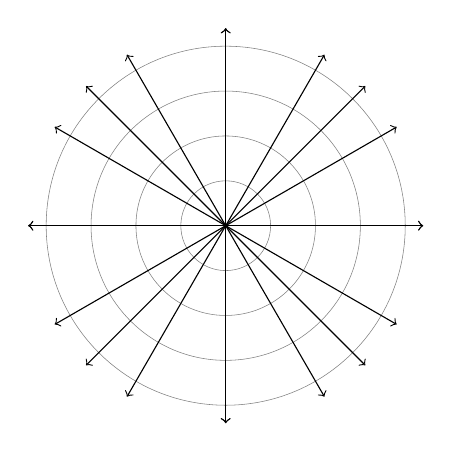
\begin{tikzpicture}[scale=0.57,baseline=(current bounding
        box.center)]
        \foreach \i in {1,2,3,4}{ \draw[help lines] (0,0) circle (\i)
          ; }

        %\foreach{\i} in {1,2,3,4}{ \draw (\i, 0) node[below
          %right]{\i}; \draw (0,\i) node[above right] {\i}; }

        \foreach \i in {30, 60, ..., 360} \draw[->] (0,0) -- (\i:4.4);

        \foreach \i in {45, 90, ..., 360} \draw[->] (0,0) -- (\i:4.4);
      \end{tikzpicture}


  \item Find the area enclosed by the inner loop.
\vskip3.15in
\vfill

\vfill
  \end{enumerate}
\end{enumerate}
\newpage
\textbf{Extra Credit} Let $f(x) = \displaystyle{\sum_{n=0}^\infty { \frac{1}{2} \choose n} \frac{x^n}{3^n}}.$
	\begin{enumerate}
	\item Determine the first 4 terms in the series. Simplify the coefficients.
	\vfill
	\item The series converges when $x=2.$ Determine the sum.
	\vfill
	\end{enumerate}
\end{document}